\documentclass[12pt]{article}
\usepackage[brazil]{babel}
\usepackage{graphicx}
\usepackage{mathtools}
\usepackage{float} 
\usepackage{xcolor}
\usepackage{amsmath, amssymb, bm}


\usepackage{array}
\usepackage{booktabs}



% margenes
\usepackage[a4paper,left=3cm,right=3cm,top=3cm]{geometry}

%opening
\title{}
\author{}

\begin{document}

\begin{center}
	{\tiny {\normalsize {\large \textbf{Convecção}\\ Lista de exercicios 5\\
	
	\textbf{Cristian Herledy Lopez Lara}}}}
\end{center}

\subsection*{Problema 5.1 livro texto}


\textbf{Mostre que a equação do momento é dominada pelos 3 termos de escala da equação 5.9.}\\

\textbf{Desenvolvimento} 

A derivação das equações constitutivas começa com a análise do problema de convecção natural em uma cavidade retangular, conforme mostrado na Figura 1.

\begin{figure}[H]
	\centering
	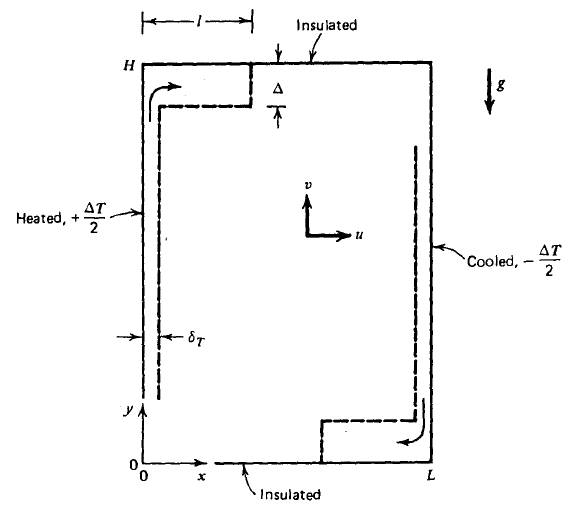
\includegraphics[width=.65\textwidth]{Figures/1_1}
	\caption{Cavidade retangular 2D com paredes isotérmicas}
\end{figure}

No instante t=0, o fluido é isotérmico e estático $u = v = 0$. As equações de conservação para massa, momento e energia serão

\begin{equation}
	\frac{\partial u}{\partial x} + \frac{\partial v}{\partial y} = 0
\end{equation}

\begin{equation}
	\frac{\partial u}{\partial t} + u \frac{\partial u}{\partial x} + v \frac{\partial u}{\partial y} = -\frac{1}{\rho} \frac{\partial P}{\partial x} + \nu \left( \frac{\partial^2 u}{\partial x^2} + \frac{\partial^2 u}{\partial y^2} \right)
\end{equation}

\begin{equation}
	\frac{\partial v}{\partial t} + u \frac{\partial v}{\partial x} + v \frac{\partial v}{\partial y} = -\frac{1}{\rho} \frac{\partial P}{\partial y} + \nu \left( \frac{\partial^2 v}{\partial x^2} + \frac{\partial^2 v}{\partial y^2} \right) - g \left[ 1 - \beta (T - T_0) \right]
\end{equation}

\begin{equation}
	\frac{\partial T}{\partial t} + u \frac{\partial T}{\partial x} + v \frac{\partial T}{\partial y} = \alpha \left( \frac{\partial^2 T}{\partial x^2} + \frac{\partial^2 T}{\partial y^2} \right)
\end{equation}

Logo após t+0, o fluido está estacionário próximo à parede lateral, então com as escalas de $\Delta T \sim T \ , \ \delta_{T} \sim x \ , \ y \sim H $,  o equilíbrio entre a inércia térmica e a condução normal à parede é governado pela relação

\begin{equation}
	\frac{\Delta T}{t} \sim \alpha \frac{\Delta T}{\delta_T^2}
\end{equation}

Quando $u = v = 0 \ $,$ \ \dfrac{\partial^{2} T}{\partial y^{2}} \ll \dfrac{\partial^{2} T}{\partial x^{2}} $ porque no instante inicial, a espessura da camada limite é muito menor que a altura da cavidade. Da equação 5 pode-se deduzir que

\begin{equation}
	\delta_T \sim (\alpha t)^{1/2}
\end{equation}

Portanto, o problema é dominado pelo movimento do fluido na direção vertical $v$. Eliminando os termos de pressão nas equações de momento, diferenciando os termos de tempo e convecção, obtemos

\begin{align}
	\frac{\partial}{\partial x} \left( \frac{\partial v}{\partial t} + u \frac{\partial v}{\partial x} + v \frac{\partial v}{\partial y} \right) - \frac{\partial}{\partial y} \left( \frac{\partial u}{\partial t} + u \frac{\partial u}{\partial x} + v \frac{\partial u}{\partial y} \right) \\
	= \nu \left[ \frac{\partial}{\partial x} \left( \frac{\partial^2 v}{\partial x^2} + \frac{\partial^2 v}{\partial y^2} \right) - \frac{\partial}{\partial y} \left( \frac{\partial^2 u}{\partial x^2} + \frac{\partial^2 u}{\partial y^2} \right) \right] + g \beta \frac{\partial T}{\partial x}
\end{align}

Nesta equação, identificamos três termos: inércia no lado direito, difusão viscosa na primeira parte do lado esquerdo e o termo empuxo no final. Aplicando as suposições para as velocidades $u = v = 0$ e multiplicando pelo $\frac{\delta_{T} t }{v}$ lado direito, obtemos a primeira análise de escala da seguinte forma:


\begin{equation}
	1 \ , \ \frac{vt}{H} \ , \  \frac{vt}{H} \ \sim \ \frac{1}{\delta_{T}} \left(  \frac{\nu v }{\delta_{T}^{2}}  \gg  \frac{\nu v }{H_{2}}\right)  \ , \     \frac{1}{H}\left(  \frac{\nu v \delta_{T} }{H}  \frac{1}{\delta_{T}^{2}}  \gg   \frac{\nu v  }{H}  \frac{\delta_{T}}{H^{2}}\right) 
\end{equation} 

Como $\frac{vt}{H} < 1 $ cuando $t \rightarrow 0$, e $\frac{\nu v }{\delta_{T}^{3}}\gg \frac{\nu v }{\delta_{T}H^{2}}$

\begin{equation}
	 \frac{v}{\delta_{T}t} \ , \  \frac{\nu v}{\delta_{T}^{3}}   \ , \ \frac{ g\beta\Delta T}{\delta_{T}}
\end{equation}

Dividindo por $\dfrac{\delta T^{3}}{\nu v}$

\begin{equation}
	\frac{\delta_{T}^{2}}{vt} \ , \ 1 \ , \ \frac{ g\beta\Delta T \delta_{T}^{2}}{\nu v}
\end{equation}

Usando (6)

\begin{equation}
	\frac{\alpha t}{vt} \ , \ 1 \ , \ \frac{ g\beta\Delta T \delta_{T}^{2}}{\nu v}
\end{equation}
\begin{equation}
	\frac{1}{Pr} \ , \ 1 \ , \ \frac{ g\beta\Delta T \delta_{T}^{2}}{\nu v}
\end{equation}

Se $Pr\gg 1$

\begin{equation}
	v \sim \frac{ g\beta\Delta T \delta_{T}^{2}}{\nu }
\end{equation}

Portanto, com a análise de escala observa-se que a força que movimenta o fluido no problema é a força de empuxo. O problema agora gira em torno do equilíbrio entre as forças de inércia e atrito com a força de empuxo.


\subsection*{Problema 5.9 livro texto}

\textbf{O grande reservatório cilíndrico mostrado na Fig. 2 está perfeitamente isolado e preenchido com água. Dois tubos horizontais com diâmetro externo de 4 cm estão posicionados no mesmo nível nas proximidades da linha central do reservatório. As temperaturas das paredes dos tubos são mantidas em \( T_1 = 30^\circ C \) e \( T_2 = 20^\circ C \) por fluxos internos de água com temperatura controlada. Calcule a taxa de transferência de calor do tubo quente para o tubo frio através do reservatório de água, assumindo que o espaço entre os tubos é suficientemente grande para que as camadas limite que revestem os tubos não se toquem (este caso está ilustrado na figura). Suponha ainda que as propriedades de temperatura da película das duas camadas limite sejam iguais às propriedades avaliadas à temperatura média do reservatório de água, \( T_\infty \). Comece com o cálculo de \( T_\infty \), e reconheça a centrosimetria do padrão de fluxo, ou seja, a simetria em torno da linha central do grande reservatório.
}\\

\begin{figure}[H]
	\centering
	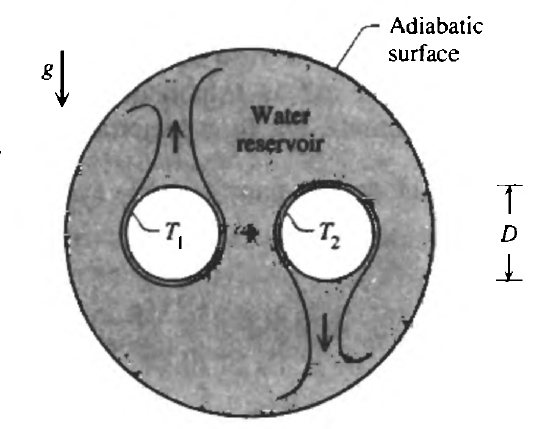
\includegraphics[width=.65\textwidth]{Figures/1_2}
	\caption{Cavidade cilindrica com tubos a temperatura $T_1$ e $T_2$ }
\end{figure}

\textbf{Desenvolvimento} 

A análise parte do estabelecimento das equações de conservação de massa, momento e energia em coordenadas cilíndricas 2D.

\begin{equation}
	\frac{\partial v_r}{\partial r} + \frac{v_r}{r} + \frac{1}{r} \frac{\partial v_\theta}{\partial \theta} = 0
\end{equation}
\begin{align}
	\rho \left( \frac{\partial v_r}{\partial t} + v_r \frac{\partial v_r}{\partial r} + \frac{v_\theta}{r} \frac{\partial v_r}{\partial \theta} - \frac{v_\theta^2}{r} + v_z \frac{\partial v_r}{\partial z} \right) = \\
	\frac{\partial P}{\partial r} + \mu \left( \frac{\partial^2 v_r}{\partial r^2} + \frac{1}{r} \frac{\partial v_r}{\partial r} - \frac{v_r}{r^2} + \frac{1}{r^{2}}\frac{\partial^2 v_r}{\partial \theta^2} - \frac{2}{r^{2}}  \frac{\partial v_\theta}{\partial \theta}  \right) + F_{r}
\end{align}

\begin{align}
	\rho \left( \frac{\partial v_\theta}{\partial t} + v_r \frac{\partial v_\theta}{\partial r} + \frac{v_\theta}{r} \frac{\partial v_\theta}{\partial \theta} + \frac{v_\theta v_{r}}{r} + v_z \frac{\partial v_\theta}{\partial z} \right) = \\
	\frac{1}{r}\frac{\partial P}{\partial \theta} + \mu \left( \frac{\partial^2 v_\theta}{\partial r^2} + \frac{1}{r} \frac{\partial v_\theta}{\partial r} - \frac{v_\theta}{r^2} + \frac{1}{r^{2}}\frac{\partial^2 v_\theta}{\partial \theta^2} + \frac{2}{r^{2}}  \frac{\partial v_r}{\partial \theta}      \right) + F_{\theta}
\end{align}

\begin{equation}
	\rho c_p \left( \frac{\partial T}{\partial t} + v_r \frac{\partial T}{\partial r} + \frac{v_\theta}{r} \frac{\partial T}{\partial \theta} \right) = k \left( \frac{1}{r} \frac{\partial}{\partial r} \left( r \frac{\partial T}{\partial r} \right) +\frac{1}{r^{2}} \frac{\partial^2 T}{\partial \theta^2} \right)
\end{equation}


Onde $F_{r} $ e $F_{\theta} $ estão associados a forças gravitacionais. Considerando condições semelhantes ao problema 5.1, onde as velocidades radial e angular são nulas no instante mais próximo de $t=0^{+}$, e tendo em conta que

\begin{align}
	T_{inf} = \frac{T_{H} - T_{C}}{2} \ e \ \delta_{t}\sim(\alpha t)^{0.5}
\end{align}

Os termos de escala para as grandezas de convecção, atrito e empuxo respetivamente são obtidos

\begin{align}
	\frac{v_{\theta}}{\delta_{T}t} \ , \ \nu \frac{v_{\theta}}{\delta_{T}^{3}} \ , \ \frac{g\beta \Delta T}{\delta_{T}}
\end{align}

Pode-se observar que a escala de velocidade é em termos de velocidade angular$v_{\theta}$. Isso ocorre porque a mudança na densidade da água direciona as camadas limites na coordenada vertical do recipiente. Portanto, o fluxo de massa será no sentido horário, e as velocidades são uma função direta da coordenada angular.\\

\begin{figure}[H]
	\centering
	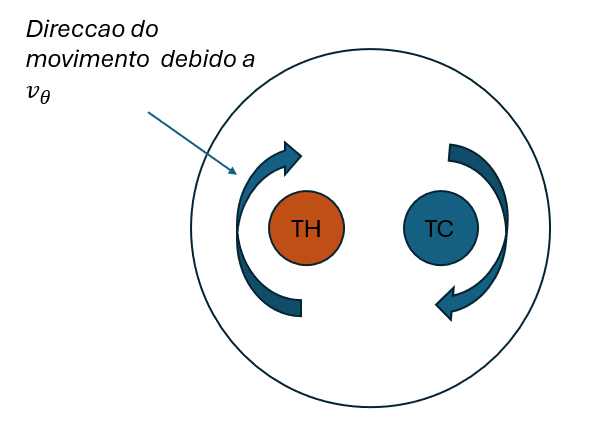
\includegraphics[width=.65\textwidth]{Figures/1_3}
	\caption{Esquema da direção do fluxo de calor dentro do recipiente }
\end{figure}

Dividindo pela escala do termo de atrito

\begin{equation}
	\frac{1}{Pr} \ , \ 1 \ , \ \frac{ g\beta\Delta T \delta_{T}^{2}}{\nu v_{\theta}}
\end{equation}

Como o calor viaja através da água, que é um fluido com $Pr\gg 1$

\begin{equation}
	v \sim \frac{ g\beta\Delta T \delta_{T}^{2}}{\nu }
\end{equation}

A partir da equação da energia, pode-se determinar que com o aumento do tempo, o balanço é em termos de


\begin{equation}
	\delta_{T}^{2}\sim \frac{\alpha H}{v} \ e \ t\sim \left( \frac{\nu D}{g\beta \Delta T \alpha}\right)^{0.5} 
\end{equation}


Portanto, em termos do número de Rayleigh será

\begin{equation}
	\delta_{T}\sim D Ra_{D}^{1/4} 
\end{equation}
Onde
\begin{equation}
	 Ra_{D}=\frac{g\beta\Delta TD^{3}}{\alpha \nu}
\end{equation}

Para o cálculo do número de Rayleigh, são utilizadas as propriedades da água $T_{inf}$.

\begin{equation}
	Ra_{D}=\frac{(9.81 m/s^{2})(0.00021 K^{-1})(10K)(0.04m)^{3}}{(0.143x10^{-6}m^{2}/s)   (0.893x10^{-6}m^{2}/s)} \ = \ 1.03 x 10^{7}
\end{equation}

Calculando a taxa de transferência de calor por unidade de comprimento

\begin{equation}
	q' = k\Delta TRa_{D}^{1/4} \ = \ 340 \  W/m
\end{equation}

Paralelamente, realizar uma validação com o cálculo do número médio de Nusselt (equação 4.122 do livro texto)


\begin{equation}
	\bar{Nu} = 35
\end{equation}
\begin{equation}
	q' = \frac{\bar{Nu}\Delta T k}{D}\frac{1}{D}  = 213 W/m 
\end{equation}

Onde o fator $1/D$ é so usado para expressar a taxa de transferência de calor por área (equação 4.123) por unidade de comprimento. \\

Conclui-se que com a expressão por correlações obtém-se uma magnitude de mesma escala que aquela obtida com a análise de escala $\sim 10^{2}$.

\begin{thebibliography}{999}
	
	
	\bibitem{abejan}
	Adrian Bejan,
	Convection Heat Transfer.
	Durham, North Carolina,
	3rd Edition,
	2004.
	
	\bibitem{Patterson}
	J. Patterson, et al,
	Unsteady natural convection in a rectangular cavity.
	J Fluid Mech.
	1980.
	
	\bibitem{Churchill}
	Churchill, et al,
	Correlating equations for laminar and turbulent convection along a vertical surface.
	J Heat Mass Transfer.
	1975.
	
\end{thebibliography}



\end{document}





